\documentclass[14pt]{extarticle}

%Russian-specific packages
\usepackage[russian]{babel}
\usepackage{cmap}
\usepackage[utf8]{inputenc}

%Hyphenation rules
\usepackage{hyphenat}

\usepackage{extsizes}

%Math
\usepackage{mathtools}
\usepackage{mathrsfs}
\usepackage{amsthm}
\usepackage{amsmath}
\usepackage{amssymb}
\usepackage{amsfonts}
\usepackage{accents}
\usepackage{systeme}
\usepackage{tikz}
\usepackage{clrscode}

\DeclareMathOperator{\rank}{rank}
\DeclareMathOperator{\im}{im}
\DeclareMathOperator{\sign}{sign}
\newcommand\aug{\fboxsep=-\fboxrule\!\!\!\fbox{\strut}\!\!\!}
%-------------------------------------- 

%Graphics
\usepackage{graphicx}
\graphicspath{{pictures/}}
\DeclareGraphicsExtensions{.pdf,.png,.jpg}
\usepackage{wrapfig}

\usepackage[a4paper,left=3cm,right=3cm,top=2cm,bottom=2cm]{geometry}
\usepackage{verbatim}
\providecommand{\tightlist}{\setlength{\itemsep}{0pt}\setlength{\parskip}{0pt}}

%Style
\usepackage[most]{tcolorbox}

\include{style.tex}

\title{Отчет по курсу прикладных математических пакетов}
\author{Соломеин Лев, КН-301}

\begin{document}
    \maketitle

    \clearpage

    \section*{Задача}

        В рамках курсовой работы я рассматриваю популяцонную модель Хасселя. Для анализа этой модели мне необходимо было построить графики функций, бифуркации и временного ряда.

    \section*{Реализация}

        Для решения данной задачи я использовал Wolfram Mathematica и Python. 
        
        На языке Python я реализовал несколько алгоритмов. Вся реализация состоит из трех файлов, в каждом файле написан алгоритм для построения одного вида графиков. Алгоритм принимает на вход некоторые параметры. Затем он расчитывает положения точек, которые далее будут нарисованы на графике.

        Перейдем ко второй части решения данной задачи. 

        Реализация на языке Mathematica состоит из двух файлов. Файл Utils.wl содержит определение пакета, в котором есть несколько функций. Есть функция, которая сохраняет отрисованный график в файл. Остальные функции нужны для построения различных видов графика. Функция, которая строит график принимат на вход массив координат точек на оси абсцисс, массив координат точек на оси ординат и путь к файлу, в котором необходимо сохранить результат.

        Во втором файле подключается пакет из файла Utils.wl. Для построения графика функций \(y = \alpha x^2\) и \(y = (\beta + x)^6\) используются встроенные средства Mathematica. 
        
        Для построения остальных графиков необходимо задействовать интерпретатор Python. Для этого необходимо указать Mathematic'e где взять интерпретатор Python. Это делается один раз. 
        
        Далее создается объект интерпретатора Python. После этого говорим Mathematic'е, откуда следует загружать скрипты на Python. Затем готовим аргументы для входных параметров. После этого вызываем код на Python, который возвращает два массива. На данном этапе у нас есть данные, которые теперь надо визуализировать. Для этого мы вызываем соответствующие функции из пакета, который я упомянул выше.

        TODO(Может быть стоит разобрать на одном примере)

        TODO(А зачем? А чтоб потом можно было вставить графики в отчет)

    \section*{Результат}

        Здесь представлены результаты работы данной программы:

        \begin{figure}[h]
            \centering
            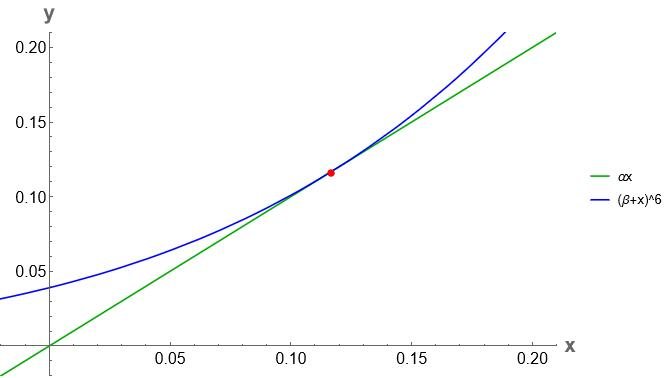
\includegraphics[width=\textwidth]{images/one_intersection.jpg}
            \caption{Одна точка пересечения}
        \end{figure}

        \begin{figure}[h]
            \centering
            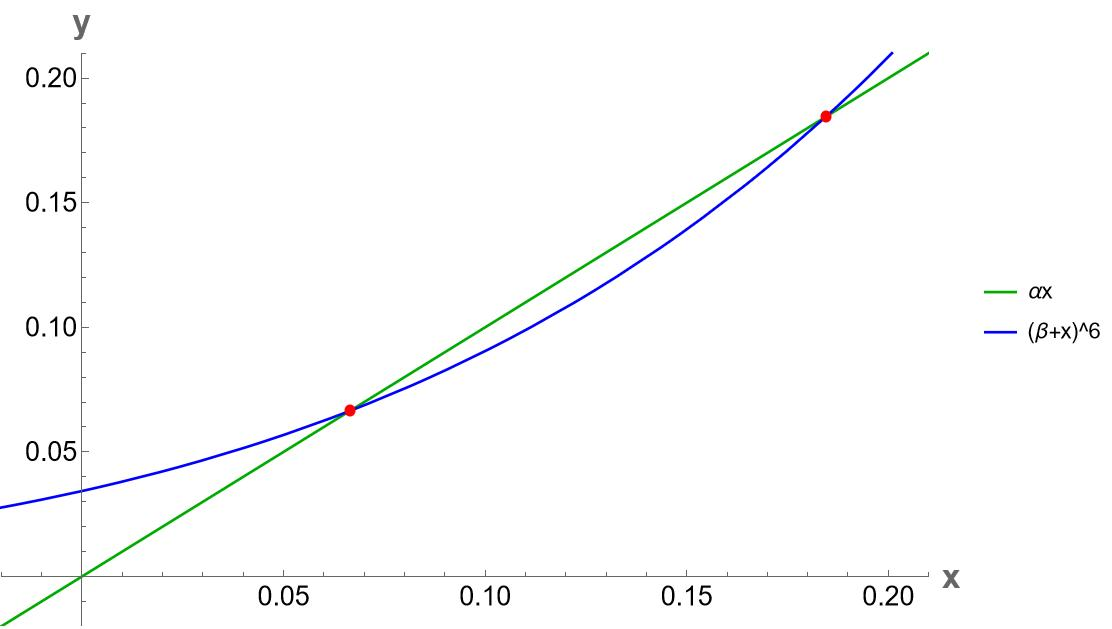
\includegraphics[width=\textwidth]{images/two_intersection.jpg}
            \caption{Две точки пересечения}
        \end{figure}

        \begin{figure}[h]
            \centering
            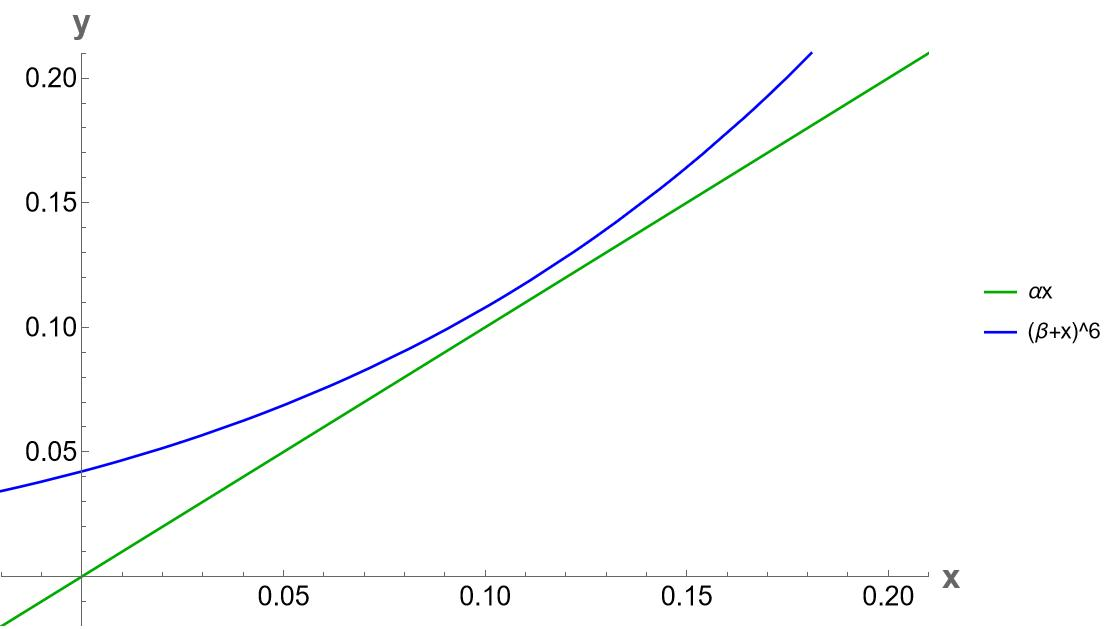
\includegraphics[width=\textwidth]{images/zero_intersection.jpg}
            \caption{Нет точек пересечения}
        \end{figure}

        \begin{figure}[h]
            \centering
            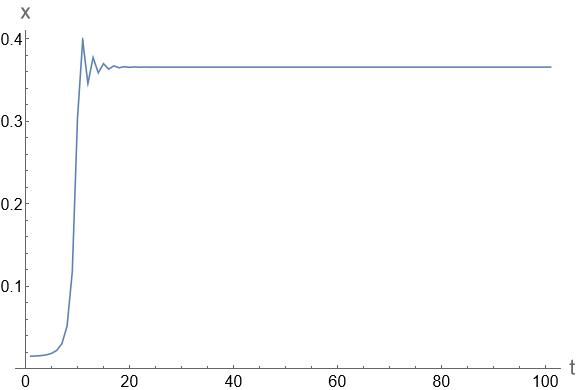
\includegraphics[width=\textwidth]{images/time_series.jpg}
            \caption{Временной ряд}
        \end{figure}

        \begin{figure}[h]
            \centering
            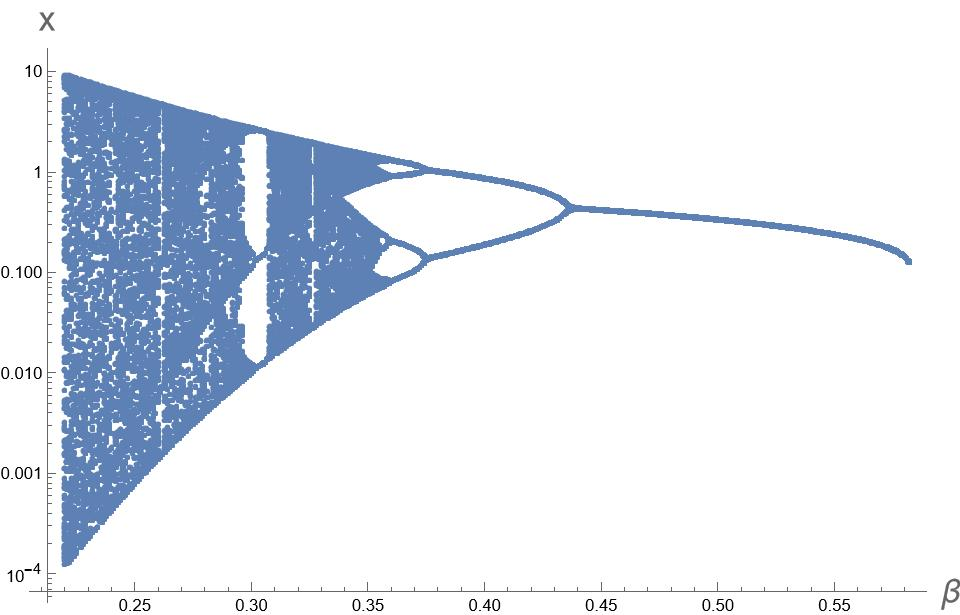
\includegraphics[width=\textwidth]{images/bifurcation.jpg}
            \caption{График бифуркации}
        \end{figure}

        \begin{figure}[h]
            \centering
            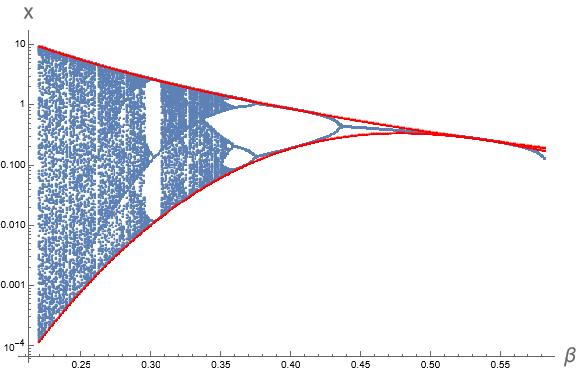
\includegraphics[width=\textwidth]{images/bifurcation_chaos.jpg}
            \caption{График бифуркации с границами хаоса}
        \end{figure}

\end{document}